\documentclass[11pt]{article}
\usepackage[final]{acl}
\usepackage{times}
\usepackage{latexsym}
\usepackage[T1]{fontenc}
\usepackage[utf8]{inputenc}
\usepackage{microtype}
\usepackage{inconsolata}
\usepackage{graphicx}
\usepackage{booktabs}
\usepackage{amsmath}
\usepackage[indonesian]{babel}
\usepackage{xurl}

\title{Qwen3.5-9B untuk StereoQueerEval:\\
Deteksi Ujaran Kebencian terhadap Komunitas LGBTQIA+\\
dengan LoRA}
\author{Draf Penelitian \\
Identitas dan afiliasi penulis belum diisi}

\begin{document}
\maketitle
\begin{abstract}
Penelitian ini menyajikan pendekatan untuk menyelesaikan Subtask B StereoQueerEval pada SemEval 2027, yaitu mengelompokkan komentar YouTube menjadi komentar nonkebencian, kebencian implisit, dan kebencian eksplisit. Qwen3.5-9B disesuaikan dengan data berlabel menggunakan Low-Rank Adaptation (LoRA). Komentar diberikan bersama penjelasan kategori, kemudian label ditentukan berdasarkan skor jawaban yang dihitung oleh model. Evaluasi dilakukan pada data Inggris, Italia, dan Belanda yang dibagi menjadi bagian pelatihan, validasi, dan pengujian. Tiga bahasa instruksi digunakan sebagai pilihan pengaturan pada setiap bahasa data. Nilai macro-F1 tertinggi yang teramati pada pengujian internal adalah 0,715757 untuk Inggris, 0,7036 untuk Italia, dan 0,641522 untuk Belanda. Pada tujuh perbandingan yang tersedia, penyesuaian model meningkatkan macro-F1 sebesar 12,47--26,94 poin dibandingkan model awal tanpa pelatihan pada data task. Analisis per kelas menunjukkan bahwa kebencian implisit masih lebih sulit dibedakan. Hasil ini merupakan evaluasi internal, bukan hasil pengujian resmi shared task.
\end{abstract}

\section{Pendahuluan}
% Evidence: L101,L102,L110.
StereoQueerEval merupakan task deteksi stereotip dan ujaran kebencian terhadap komunitas LGBTQIA+ dalam komentar YouTube berbahasa Inggris, Italia, Belanda, dan Persia \citep{stereoqueereval-2026-data}. Salah satu tugasnya adalah membedakan komentar nonkebencian, kebencian implisit, dan kebencian eksplisit. Pembedaan ini memerlukan pemahaman makna, karena kebencian dapat disampaikan melalui ungkapan tidak langsung atau bahasa tersandi \citep{elsherief-etal-2021-latent}. Stereotip juga perlu dibedakan dari ujaran kebencian; QUEEREOTYPES memberikan anotasi terpisah untuk kedua hal tersebut \citep{cignarella-etal-2024-queereotypes}.

% Evidence: L111,L112.
Model bahasa besar atau large language model (LLM) telah digunakan untuk mengenali teks anti-LGBTQIA+. \citet{chan-etal-2024-hate} membandingkan GPT-3.5-turbo sebelum dan setelah penyesuaian pada data berlabel, serta melaporkan perbaikan hasil pada beberapa bahasa. \citet{nguyen-etal-2025-leveraging} mengevaluasi lima LLM tanpa pelatihan tambahan pada data yang diuji dan menunjukkan bahwa kesalahan pengenalan konten masih terjadi. Temuan tersebut menjadi dasar untuk membandingkan model awal dengan model yang telah disesuaikan pada data task.

% Evidence: Q001,Q004,L103,L104.
Penelitian ini menggunakan Qwen3.5-9B \citep{qwen-team-2026-qwen35} dengan pelatihan pada data berlabel, yang disebut supervised fine-tuning (SFT). Penyesuaian dilakukan melalui LoRA, yaitu metode yang melatih sejumlah kecil parameter tambahan sambil mempertahankan bobot utama model \citep{hu-etal-2021-lora}. Setiap komentar diberikan bersama definisi tiga kategori. Model kemudian memilih satu jawaban yang mewakili label komentar.

% Evidence: Q001,Q002,Q003,Q004,Q006.
Evaluasi mencakup sembilan pasangan bahasa data dan instruksi pada Inggris, Italia, dan Belanda. Perbandingan dengan model awal serta analisis kelas digunakan untuk menilai kemampuan klasifikasi dan kesalahan yang masih perlu diperbaiki.

\section{Deskripsi Task}
% Evidence: Q001,Q005,L110.
Subtask B StereoQueerEval meminta pemberian satu label ujaran kebencian untuk setiap komentar. Label \texttt{no} menunjukkan komentar nonkebencian, \texttt{yes\_implicit} menunjukkan kebencian yang disampaikan secara tidak langsung, dan \texttt{yes\_explicit} menunjukkan kebencian yang dinyatakan secara langsung. Ketiga kategori mengikuti label yang disediakan penyelenggara \citep{stereoqueereval-2026-data}.

% Evidence: Q001,Q005,Q006.
Data juga menyediakan judul dan deskripsi video serta anotasi stereotip dan target kebencian. Penelitian ini menggunakan teks komentar dan penanda bahasa sebagai masukan, sedangkan label lain tidak dijadikan petunjuk prediksi. Cakupan evaluasi dibatasi pada tiga bahasa yang memiliki data pelatihan dalam percobaan ini, yaitu Inggris (EN), Italia (IT), dan Belanda (NL).

\section{Penelitian Terkait}
\subsection{Deteksi Kebencian terhadap LGBTQIA+}
% Evidence: L108,L114.
\citet{nozza-2022-nozza} menggunakan BERT, RoBERTa, dan HateBERT yang dilatih pada komentar YouTube Inggris untuk mendeteksi homofobia dan transfobia. Prediksi beberapa model digabungkan melalui pemungutan suara. \citet{wong-etal-2023-cantnlp} menggunakan XLM-R yang dilatih kembali pada teks media sosial sebelum disesuaikan untuk klasifikasi dalam beberapa bahasa. Kedua penelitian menunjukkan penggunaan model bahasa untuk mengenali kebencian terhadap kelompok yang menjadi sasaran task ini.

% Evidence: L111.
\citet{chan-etal-2024-hate} mengevaluasi GPT-3.5-turbo pada data Inggris, Italia, Tionghoa, dan Inggris--Tamil. Percobaan mencakup teks asli dan teks yang diterjemahkan ke Inggris, dengan maupun tanpa penyesuaian model. Penelitian tersebut mendukung penggunaan data berlabel untuk meningkatkan klasifikasi multilingual. Namun, tugasnya hanya membedakan dua kelas dan hasilnya dilaporkan sebagai weighted-F1. Penelitian ini membedakan tiga kelas dan memakai macro-F1, sehingga kedua hasil tidak dibandingkan langsung.

% Evidence: L112.
\citet{nguyen-etal-2025-leveraging} mengevaluasi lima LLM untuk klasifikasi biner anti-LGBTQIA+ tanpa pelatihan tambahan, termasuk kesalahan dan ketepatan tingkat keyakinannya. Penelitian ini menggunakan pelatihan berlabel dan menambahkan pembedaan kebencian implisit dari eksplisit.

\subsection{Penyesuaian Model untuk Klasifikasi}
% Evidence: L104,L113.
Pada SemEval-2023 Task 10, JUAGE menggunakan soft prompt-tuning untuk klasifikasi seksisme \citep{sorensen-etal-2023-juage}. Pendekatan tersebut mempertahankan bobot utama model dan mempelajari representasi instruksi dari data berlabel. LoRA menawarkan cara penyesuaian yang berbeda, yaitu mempelajari perubahan berukuran kecil pada parameter model \citep{hu-etal-2021-lora}. Penelitian ini memilih LoRA untuk menyesuaikan Qwen3.5-9B pada label StereoQueerEval.

\section{Pendekatan Penyelesaian}
\subsection{Tahapan Klasifikasi}
% Evidence: Q001,Q004,Q006.
Penyelesaian meliputi penyusunan instruksi kategori, pelatihan menggunakan komentar berlabel, dan pemilihan label berdasarkan skor jawaban. Bentuk masukan serta aturan penentuan label dipertahankan selama pelatihan dan pengujian.

\subsection{Penyesuaian Qwen3.5-9B dengan LoRA}
% Evidence: Q001,Q004,L103,L104.
Qwen3.5-9B merupakan model bahasa yang dapat memproses instruksi dan teks masukan \citep{qwen-team-2026-qwen35}. Dalam penelitian ini, penggunaannya dibatasi pada komentar berbentuk teks. LoRA memungkinkan penyesuaian melalui parameter tambahan tanpa melatih ulang seluruh bobot utama \citep{hu-etal-2021-lora}. Catatan pelatihan menunjukkan bahwa sekitar 0,48\% dari parameter yang dimuat dapat diperbarui.

% Evidence: Q001,Q004.
Pelatihan diarahkan pada jawaban yang benar, bukan pada pengulangan instruksi atau komentar. Dengan cara ini, model belajar menghubungkan isi komentar dengan kategori yang sesuai. Hasil pelatihan yang digunakan untuk pengujian dipilih berdasarkan nilai macro-F1 tertinggi pada data validasi.

\subsection{Penyusunan Instruksi dan Jawaban}
% Evidence: Q001,Q004,Q006.
Instruksi tersedia dalam bahasa Inggris, Italia, dan Belanda. Isinya menjelaskan kategori komentar nonkebencian, kebencian eksplisit, dan kebencian implisit, serta meminta satu jawaban angka tanpa penjelasan tambahan. Instruksi juga menegaskan bahwa penyebutan identitas LGBTQIA+ saja tidak cukup untuk menganggap komentar sebagai kebencian. Tidak ada contoh komentar berlabel di dalam instruksi.

Jawaban angka dipetakan sebagai berikut: 0 untuk \texttt{no}, 1 untuk \texttt{yes\_explicit}, dan 2 untuk \texttt{yes\_implicit}. Setelah prediksi diperoleh, angka dikembalikan ke label asli untuk evaluasi. Komentar dipertahankan dalam bahasa aslinya, termasuk kapitalisasi dan emoji. Penanda nama bahasa dan komentar pada masukan tetap menggunakan bahasa Inggris.

\subsection{Penentuan Label}
% Evidence: Q001,Q004.
Untuk setiap komentar, model menghitung skor tiga pilihan jawaban. Skor berasal dari jumlah log probabilitas jawaban beserta penanda akhirnya. Pilihan dengan skor tertinggi menjadi label prediksi. Aturan ini membatasi jawaban pada tiga kategori task dan digunakan secara sama pada model awal maupun model yang telah dilatih.

\section{Pengaturan Eksperimen}
\subsection{Dataset dan Pembagian Data}
% Evidence: Q005.
Data yang digunakan berjumlah 2.989 komentar Inggris, 2.400 Italia, dan 2.238 Belanda. Setiap bahasa dibagi menjadi data pelatihan, validasi, dan pengujian dengan perbandingan mendekati 70:10:20. Pembagian menggunakan nilai awal acak atau seed 42 dan mempertahankan kelompok komentar dari konteks video yang sama serta komentar duplikat dalam bagian yang sama. Karena kelompok tidak dipecah, jumlah akhirnya tidak selalu tepat mengikuti rasio tersebut.

\begin{table}[t]
\centering
\small
\setlength{\tabcolsep}{3pt}
\begin{tabular}{llrrrr}
\toprule
Bahasa & Bagian & $N$ & no & impl. & ekspl. \\
\midrule
EN & train & 2111 & 983 & 546 & 582 \\
EN & val & 292 & 147 & 70 & 75 \\
EN & test & 586 & 277 & 156 & 153 \\
IT & train & 1699 & 822 & 401 & 476 \\
IT & val & 220 & 105 & 56 & 59 \\
IT & test & 481 & 233 & 124 & 124 \\
NL & train & 1556 & 784 & 335 & 437 \\
NL & val & 226 & 109 & 55 & 62 \\
NL & test & 456 & 234 & 97 & 125 \\
\bottomrule

\end{tabular}
\caption{Jumlah komentar pada setiap bagian data. impl. dan ekspl. merujuk pada kebencian implisit dan eksplisit; train, val, dan test masing-masing berarti pelatihan, validasi, dan pengujian.}
\label{tab:data}
\end{table}

Kelas \texttt{no} merupakan kelas terbesar pada seluruh bagian data (Tabel~\ref{tab:data}). Pemeriksaan tidak menemukan komentar yang sama setelah normalisasi maupun pasangan judul--deskripsi video yang sama pada bagian berbeda. Judul dan deskripsi digunakan sebagai pendekatan untuk mengenali kelompok video, sehingga belum menjamin bahwa setiap identitas video terpisah secara sempurna.

% Evidence: Q001,Q005,L110.
Seluruh bagian data berasal dari data pelatihan yang dirilis penyelenggara. Oleh karena itu, pengujian pada penelitian ini disebut pengujian internal. Data pelatihan digunakan untuk menyesuaikan model, data validasi untuk memilih hasil pelatihan terbaik, dan data pengujian untuk menghitung hasil akhir.

\subsection{Pelatihan dan Pilihan Pengaturan}
% Evidence: Q001,Q002,Q004,Q006.
Percobaan mencakup sembilan pasangan dari tiga bahasa data dan tiga bahasa instruksi. Setiap pasangan memulai pelatihan dari model dasar yang sama dengan parameter tambahan LoRA yang baru. Instruksi yang dipilih digunakan secara konsisten pada data pelatihan, validasi, dan pengujian. Data dari bahasa yang berbeda tidak digabungkan selama pelatihan.

% Evidence: Q001,Q004,L109.
Pelatihan menggunakan AdamW \citep{loshchilov-hutter-2019-decoupled} selama paling banyak lima putaran atau epoch pada satu GPU NVIDIA H200. Evaluasi dilakukan setelah setiap putaran. Pelatihan dihentikan lebih awal apabila macro-F1 validasi tidak membaik dalam dua evaluasi berturut-turut. Tabel~\ref{tab:hyper} menyajikan pengaturan utama agar percobaan dapat ditelusuri.

\begin{table}[t]
\centering
\small
\begin{tabular}{ll}
\toprule
Pengaturan & Nilai \\
\midrule
Seed & 42 \\
Putaran pelatihan maksimum & 5 \\
Learning rate & $10^{-4}$ \\
Ukuran batch efektif & 16 \\
Batas panjang masukan & 1.024 token \\
LoRA rank / alpha & 16 / 32 \\
LoRA dropout & 0,05 \\
Presisi perhitungan & BF16 \\
\bottomrule
\end{tabular}
\caption{Pengaturan utama pelatihan. Batch efektif adalah jumlah contoh per pembaruan parameter; token merupakan satuan potongan teks yang diproses model.}
\label{tab:hyper}
\end{table}

% Evidence: Q001,Q004.
Panjang masukan dibatasi menjadi 1.024 token, termasuk instruksi dan jawaban. Jika melebihi batas, isi pesan komentar dipotong dengan tetap menyediakan ruang untuk instruksi dan pilihan jawaban. Pembandingnya adalah model awal dalam pengaturan zero-shot, yaitu menggunakan definisi kategori tanpa pelatihan pada data task ini.

\subsection{Metrik Evaluasi}
% Evidence: Q001,Q002,Q003,Q004.
Ukuran utama adalah macro-F1, yaitu rata-rata F1 dari tiga kelas dengan bobot yang sama. Nilai ini dipilih agar penilaian tidak didominasi kelas dengan jumlah komentar terbanyak. Precision menunjukkan proporsi prediksi suatu kelas yang benar, sedangkan recall menunjukkan proporsi contoh kelas tersebut yang berhasil dikenali. Hasil kedua ukuran ini disajikan bersama jumlah contoh untuk memperjelas kemampuan setiap kelas.

Sembilan nilai macro-F1 dilaporkan pada tabel utama. Rincian prediksi untuk pasangan EN/EN dan IT/IT belum tersedia, sehingga kedua nilai tersebut hanya bersumber dari ringkasan hasil. Perbandingan dengan zero-shot dibatasi pada tujuh pasangan yang memiliki nilai pembanding.

\section{Hasil dan Pembahasan}
\subsection{Hasil pada Tiga Bahasa}
% Evidence: Q002,Q003.
Tabel~\ref{tab:main} menyajikan hasil pengujian internal. Pada data Inggris, nilai tertinggi adalah 0,715757 dengan instruksi Italia. Pada data Italia, nilai tertinggi adalah 0,7036 dengan instruksi Inggris. Pada data Belanda, nilai tertinggi adalah 0,641522 dengan instruksi Belanda.

\begin{table}[t]
\centering
\small
\setlength{\tabcolsep}{4pt}
\begin{tabular}{lrrr}
\toprule
Data & Instruksi EN & Instruksi IT & Instruksi NL \\
\midrule
EN & \textbf{0.719146} & 0.715757 & 0.688340 \\
IT & \textbf{0.7036} & 0.702038$^{\dagger}$ & 0.701449 \\
NL & 0.629927 & 0.630810 & \textbf{0.641522} \\
\bottomrule

\end{tabular}
\caption{Macro-F1 pengujian internal. Cetak tebal menunjukkan nilai tertinggi pada setiap bahasa data. $\dagger$: nilai bersumber dari ringkasan hasil tanpa rincian prediksi.}
\label{tab:main}
\end{table}

Hasil terbaik Inggris dan Italia berada di atas 0,70, sedangkan hasil terbaik Belanda masih lebih rendah. Perbedaan tersebut perlu dibaca bersama perbedaan jumlah data pelatihan dan isi komentar pada setiap bahasa. Angka ini belum cukup untuk menyimpulkan bahwa suatu bahasa secara umum lebih sulit daripada bahasa lainnya.

Tidak ada satu bahasa instruksi yang memberikan hasil tertinggi pada seluruh bahasa data. Pada Italia, ketiga pilihan menghasilkan nilai yang berdekatan, yaitu 0,701449--0,7036. Seluruh hasil dilaporkan untuk menunjukkan pilihan pengaturan yang telah dicoba. Nilai tertinggi pada data pengujian bersifat deskriptif; penetapan pilihan akhir untuk pengujian berikutnya perlu dilakukan menggunakan data validasi.

\subsection{Perbandingan dengan Model Awal}
% Evidence: Q003,Q004.
Pada tujuh pasangan yang memiliki hasil pembanding, model setelah SFT memperoleh macro-F1 lebih tinggi daripada model awal (Gambar~\ref{fig:baseline}). Kenaikannya berkisar 12,47--26,94 poin pada skala F1 0--100. Sebagai contoh, pada data Inggris dengan instruksi Belanda, macro-F1 meningkat dari 0,418932 menjadi 0,688340. Hasil ini menunjukkan manfaat pelatihan dengan label task pada percobaan yang dilakukan.

\begin{figure*}[t]
\centering
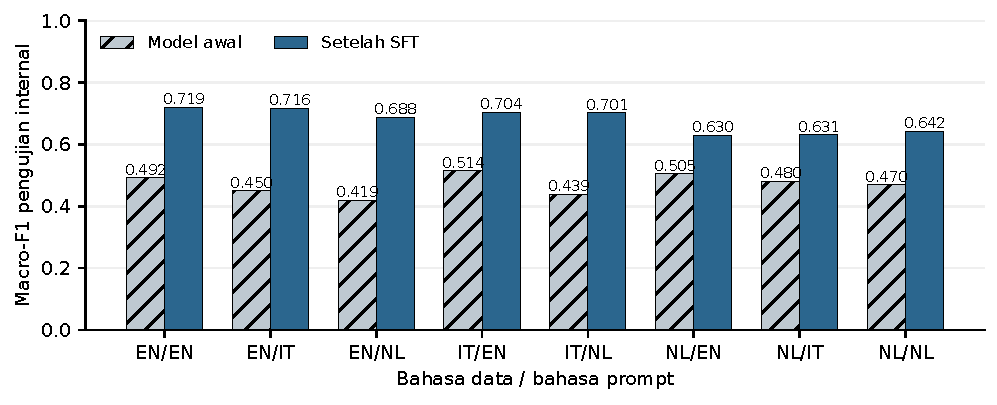
\includegraphics[width=\textwidth]{figures/qwen_sft_baseline.pdf}
\caption{Macro-F1 model awal (zero-shot) dan model setelah SFT. Label mendatar menunjukkan bahasa data/bahasa instruksi. Jumlah komentar uji: EN 586, IT 481, NL 456. Hasil EN/EN dan IT/IT tidak disertakan karena nilai zero-shot belum tersedia.}
\label{fig:baseline}
\end{figure*}

% Evidence: Q003,Q004,L111.
Perbaikan setelah penyesuaian pada data berlabel juga dilaporkan oleh \citet{chan-etal-2024-hate}. Kesamaan tersebut menjadi dukungan kualitatif bagi pendekatan pelatihan yang digunakan, dengan tetap memperhatikan perbedaan model, data, jumlah kelas, dan metrik evaluasi.

\subsection{Hasil Berdasarkan Kelas}
% Evidence: Q003,Q004.
Analisis per kelas menggunakan instruksi Belanda pada ketiga bahasa data agar pilihan instruksi tetap sama. Tabel~\ref{tab:classes} menunjukkan bahwa F1 kelas nonkebencian paling tinggi, sedangkan F1 kebencian implisit paling rendah. Nilai F1 implisit adalah 0,5397 pada Inggris, 0,6020 pada Italia, dan 0,4828 pada Belanda.

\begin{table*}[t]
\centering
\begin{tabular}{llrrrr}
\toprule
Data & Kelas & Jumlah & Precision & Recall & F1 \\
\midrule
EN & \texttt{no} & 277 & 0.8163 & 0.8339 & 0.8250 \\
EN & \texttt{yes\_implicit} & 156 & 0.5346 & 0.5449 & 0.5397 \\
EN & \texttt{yes\_explicit} & 153 & 0.7222 & 0.6797 & 0.7003 \\
IT & \texttt{no} & 233 & 0.8450 & 0.7253 & 0.7806 \\
IT & \texttt{yes\_implicit} & 124 & 0.5143 & 0.7258 & 0.6020 \\
IT & \texttt{yes\_explicit} & 124 & 0.7830 & 0.6694 & 0.7217 \\
NL & \texttt{no} & 234 & 0.8341 & 0.7949 & 0.8140 \\
NL & \texttt{yes\_implicit} & 97 & 0.4148 & 0.5773 & 0.4828 \\
NL & \texttt{yes\_explicit} & 125 & 0.7143 & 0.5600 & 0.6278 \\
\bottomrule

\end{tabular}
\caption{Hasil setiap kelas dengan instruksi Belanda. Jumlah menunjukkan banyaknya komentar dengan label sebenarnya. Precision dan recall masing-masing menjelaskan ketepatan prediksi kelas dan cakupan contoh yang dikenali.}
\label{tab:classes}
\end{table*}

Nilai F1 implisit yang rendah tidak selalu disebabkan banyaknya contoh yang terlewat. Pada Italia, recall implisit mencapai 0,7258, tetapi precision hanya 0,5143. Artinya, cukup banyak contoh implisit dikenali, namun banyak komentar kelas lain juga keliru dimasukkan ke kategori ini. Pada Belanda, precision implisit sebesar 0,4148 menunjukkan persoalan serupa. Perbaikan perlu mencakup pengenalan contoh implisit sekaligus pengurangan prediksi implisit yang keliru.

\subsection{Analisis Kesalahan Klasifikasi}
% Evidence: Q003,Q004.
Matriks kesalahan pada Gambar~\ref{fig:confusion} memperlihatkan pasangan kelas yang sering tertukar. Dengan instruksi Belanda, terdapat 166 kesalahan dari 586 komentar Inggris, 139 dari 481 komentar Italia, dan 144 dari 456 komentar Belanda. Pada Inggris, 40 komentar implisit dianggap nonkebencian dan 31 dianggap eksplisit.

\begin{figure*}[t]
\centering
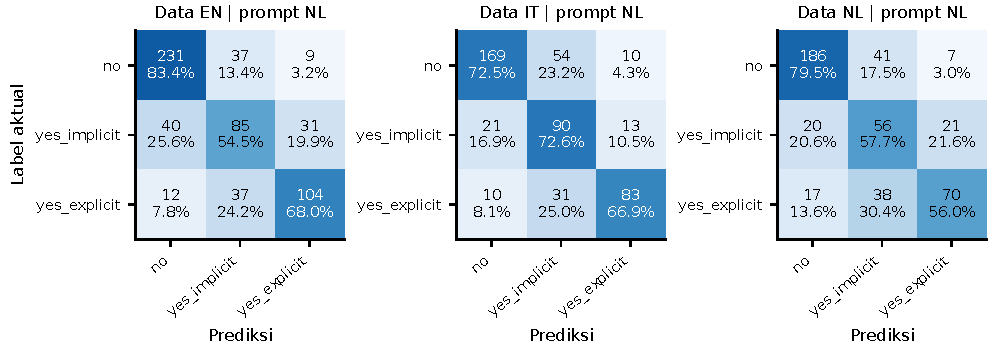
\includegraphics[width=\textwidth]{figures/qwen_confusion_nl.pdf}
\caption{Matriks kesalahan prediksi dengan instruksi Belanda. Baris menunjukkan label sebenarnya dan kolom menunjukkan prediksi. Setiap sel memuat jumlah komentar serta persentase terhadap jumlah pada baris yang sama.}
\label{fig:confusion}
\end{figure*}

Pada Italia, 54 komentar nonkebencian dan 31 komentar eksplisit keliru dimasukkan ke kelas implisit. Pada Belanda, kesalahan ke kelas implisit berasal dari 41 komentar nonkebencian dan 38 komentar eksplisit. Pola ini membantu menjelaskan precision implisit yang rendah pada kedua bahasa tersebut.

% Evidence: Q003,Q004,L102,L107.
Jumlah kesalahan belum menjelaskan penyebab pada setiap komentar. Pemeriksaan lebih lanjut dapat diarahkan pada ungkapan tidak langsung, negasi, kutipan, dan tanggapan yang menolak kebencian. HateCheck menyediakan contoh pengujian terarah untuk mengenali kelemahan semacam ini \citep{rottger-etal-2021-hatecheck}, sedangkan Latent Hatred memberikan dasar pembahasan kebencian implisit \citep{elsherief-etal-2021-latent}. Pemeriksaan tersebut merupakan pengembangan lanjutan.

\section{Kesimpulan}
% Evidence: Q001,Q002,Q003,Q004.
Qwen3.5-9B yang disesuaikan dengan LoRA digunakan untuk klasifikasi tiga kelas pada Subtask B StereoQueerEval. Nilai macro-F1 pengujian internal tertinggi yang teramati adalah 0,715757 pada Inggris, 0,7036 pada Italia, dan 0,641522 pada Belanda.

Pelatihan berlabel menghasilkan nilai lebih tinggi daripada model awal pada seluruh tujuh perbandingan yang tersedia. Meskipun demikian, pembedaan kebencian implisit masih menjadi tantangan, terutama karena komentar dari kelas lain dapat keliru dianggap implisit. Pengembangan berikutnya perlu memperkuat pembedaan antar-kelas, mengulang percobaan dengan beberapa seed, dan memilih pengaturan melalui data validasi sebelum pengujian lanjutan.

\section*{Keterbatasan}
% Evidence: Q001,Q002,Q003,Q004,Q005,Q006,L110.
Percobaan menggunakan satu seed dan satu versi instruksi per bahasa, sehingga konsistensi hasil pada pengulangan lain belum diketahui. Pengujian dilakukan pada pembagian internal data yang dirilis penyelenggara, bukan pada data uji resmi. Sebagian hasil hanya memiliki nilai ringkasan dan belum dilengkapi rincian prediksi. Analisis per kelas dibatasi pada pilihan instruksi Belanda; hasil tersebut belum mewakili seluruh pilihan instruksi.

Data berasal dari komentar YouTube bertopik LGBTQIA+, sehingga penerapannya pada platform atau topik lain masih memerlukan evaluasi. Penggunaan data mengikuti ketentuan penyelenggara \citep{stereoqueereval-2026-data}. Pemeriksaan kesalahan secara langsung pada komentar juga diperlukan untuk memahami batas penggunaan model secara lebih baik.

\bibliography{references}
\end{document}
